\textbf{COLUNI 2018 -- Questão 30}\par\medskip Em diferentes estágios do ciclo celular a molécula de DNA (Ácido Desoxirribonucléico) apresenta diferentes níveis de condensação (enrolamento), conforme representado nas figuras abaixo.



\begin{figure}[htbp]
\centering
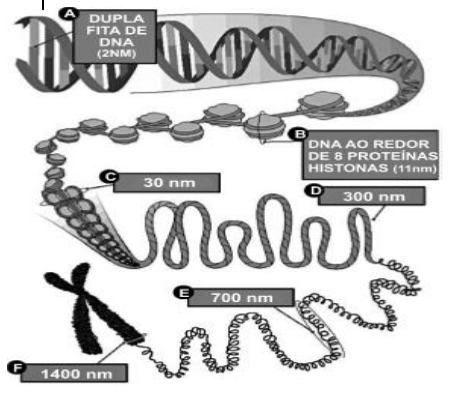
\includegraphics[width=0.48\linewidth]{static/simulados/coluni/figuras/2018/questao-30/figura-1.png}
\hfill
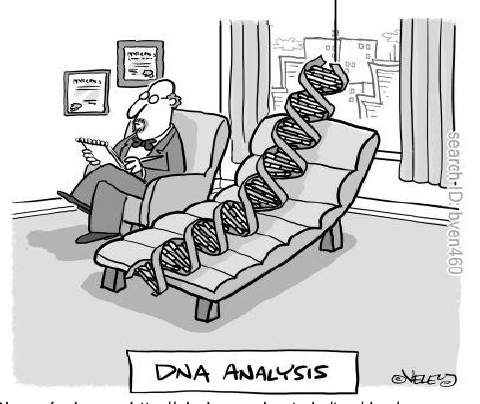
\includegraphics[width=0.48\linewidth]{static/simulados/coluni/figuras/2018/questao-30/figura-2.png}
\end{figure}
\begin{minipage}{0.48\linewidth}Disponível em: <http://piadasnerds.etc.br/tag/dna/>. Acesso em: 19 set. 2017.\end{minipage}\hfill
\begin{minipage}{0.48\linewidth}Disponível em: <https://biotergernibhi.wordpress.com/2010/10/30/adnaren-egitura-mailak-3/>. Acesso em: 19 set. 2017.\end{minipage}

Na análise de uma molécula de DNA, presente em uma célula humana, visualizou-se o material genético no nível “F” de condensação. Tal observação nos leva a deduzir que nesta célula estaria ocorrendo o processo de:


\begin{enumerate}
\item produção de ácido ribonucléico.
\item divisão celular.
\item duplicação do material genético.
\item síntese de proteínas.
\end{enumerate}
